\section{Parse Trees}

\begin{multicols}{2}
\setlength{\columnsep}{1.5cm}
\setlength{\columnseprule}{0.2pt}

Let $G$ be a context-free grammar. A string $w \in L(G)$ may have many derivations in $G$. For example, if $G$ is the context-free grammar that generates the language of balanced parentheses, then the string $()()$ can
be derived from $S$ by at least two distinct derivations, namely,
\begin{equation*}
    S \Rightarrow SS \Ra (S)S \Ra ()S \Ra ()(S) \Ra ()()
\end{equation*}
and
\begin{equation*}
    S \Rightarrow SS \Ra S(S) \Ra (S)(S) \Ra (S)() \Ra ()()
\end{equation*}
However, these two derivations are in a sense ``the same''. The rules used are the same, and they are applied at the same places in the intermediate string. The only difference is in the order in which the rules are applied. Intuitively, both derivations can be pictured as in Figure 2.
\begin{figure}[H]
    \centering
    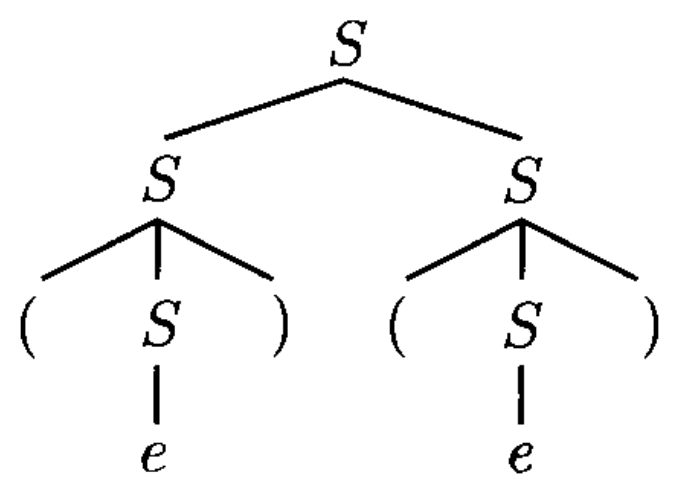
\includegraphics[width=.2\textwidth]{img/fig3-2.png}
    \caption{}
\end{figure}

We call such a picture a \textbf{parse tree}. The points are called \textbf{nodes}; each node carries a \textbf{label} that is a symbol in $V$. The topmost node is called the \textbf{root}, and the nodes along the bottom are called \textbf{leaves}. All leaves are labeled by \textit{terminals}, or possibly the empty string $e$. By concatenating the labels of the leaves from left to right, we obtain the derived string of terminals, which is
called the \textbf{yield} of the parse tree.

%% Add definition after drawing with tikz

More formally, for an arbitrary context-free grammar $G = (V, \Sigma, R, S)$, we define its parse trees and their roots, leaves, and yields, as follows.

\begin{enumerate}
    \item
        \begin{equation*}
            \circ\ a
        \end{equation*}
        This is a parse tree for each $a \in \Sigma$. The single node of this parse tree is both the root and a leaf. The yield of this parse tree is $a$.
    
    \item If $A \ra e$ is a rule in $R$, then % Later draw with tikz
        \begin{figure}[H]
            \centering
            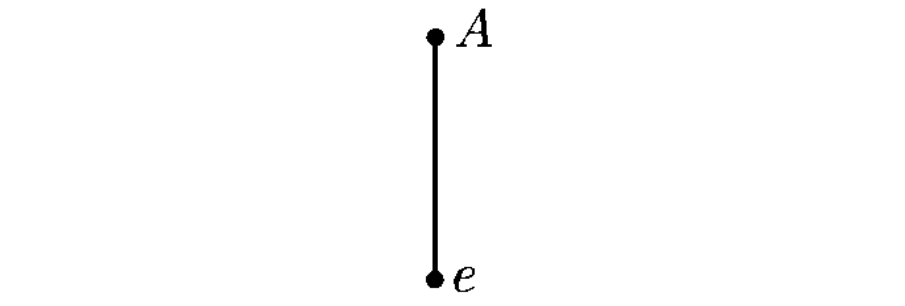
\includegraphics[width=.4\textwidth]{img/parse-tree-2.png}
        \end{figure}
        is a parse tree; its root is the node labeled $A$, its sole leaf is the node labeled $e$, and its yield is $e$.
    
    \item If
        \begin{figure}[H]
            \centering
            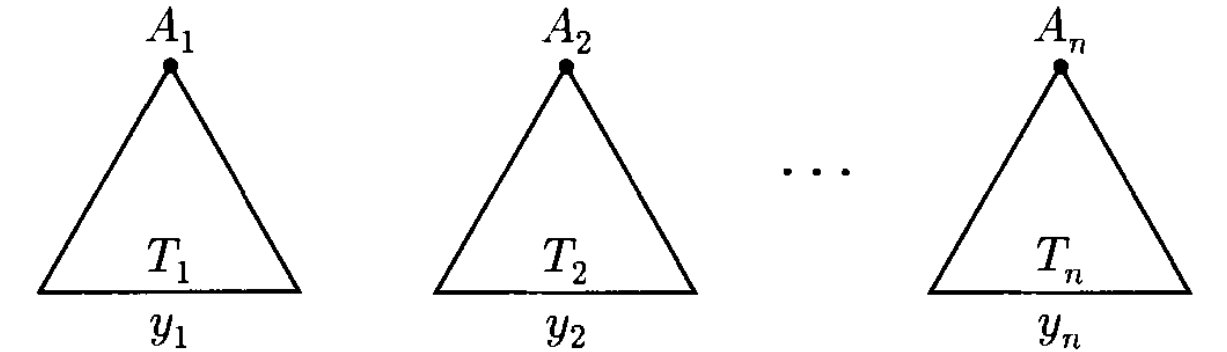
\includegraphics[width=.4\textwidth]{img/parse-tree-3.png}
        \end{figure}
        are parse trees, where $n > 1$, with roots labeled $A_1, \ldots, A_n$ respectively, and with yields $y_1, \ldots, y_n$, and $A \ra A_1 \ldots A_n$ is a rule in $R$, then
        \begin{figure}[H]
            \centering
            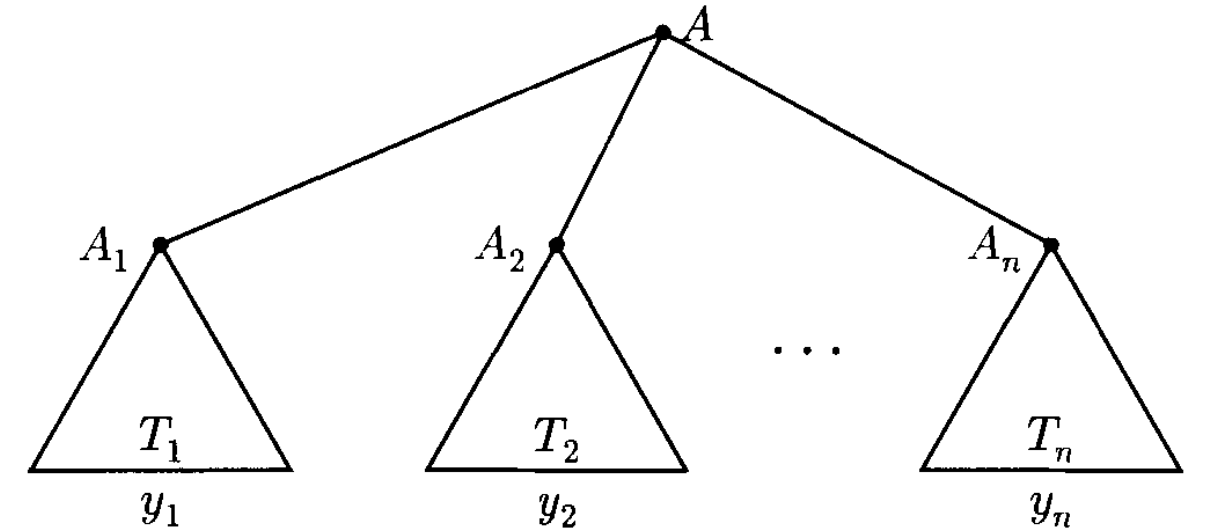
\includegraphics[width=.4\textwidth]{img/parse-tree-4.png}
        \end{figure}
        is a parse tree. Its root is the new node labeled $A$, its leaves are the leaves of its constituent parse trees, and its yield is $y_1 \ldots y_n$.
    
    \item Nothing else is a parse tree.
\end{enumerate}

Intuitively, parse trees are ways of representing derivations (\textit{the process of deriving a string}) of strings in $L(G)$ so that the superficial differences between derivations, owing to the order of application of rules, are suppressed. To put it otherwise, parse trees represent
equivalence classes of derivations. We make this intuition precise below. 

Let $G = (V, \Sigma, R, S)$ be a context-free grammar, and let $D = x_1 \Ra x_2 \Ra \cdots \Ra x_n$ and $D' = x_1' \Ra x_2' \Ra \cdots \Ra x_n'$ be two derivations in $G$, where $x_i, x_i' \in V^*$ for $i = 1, \ldots, n$; $x_1, x_1' \in V - \Sigma$; and $x_n, x_n' \in \Sigma^*$. That is, they are both derivations of terminal strings from a single nonterminal. We say that $D$ \textbf{precedes} $D'$, written $D \prec D'$, if $n > 2$ and there is an integer $k$, $1 < k < n$ such that

\begin{enumerate}
    \item for all $i \neq k$ we have $x_i = x_i'$;
    \item $x_{k-1} = x_{k-1}' = uAvBw$, where $u, v, w \in V^*$, and $A, B \in V - \Sigma$;
    \item $x_k = uyvBw$, where $A \ra y \in R$;
    \item $x_k' = uAvzw$, where $B \ra y \in R$;
    \item $x_{k+1} = x_{k+1}' = uyvzw$.
\end{enumerate}

In other words, the two derivations are identical except for two consecutive steps, during which the same two nonterminals are replaced by the same two strings \textit{but in opposite orders in the two derivations}. The derivation in which the leftmost of the two nonterminals is replaced first is said to precede the other.

\end{multicols}

\begin{example}{}
    Consider the following three derivations $D_1$ , $D_2$ , and $D_3$ in the grammar $G$ generating all strings of balanced parentheses:
    \begin{align*}
        D_1 &= S \Ra SS \Ra (S)S \Ra ((S))S \Ra (())S \Ra (())(S) \Ra (())()\\
        D_2 &= S \Ra SS \Ra (S)S \Ra ((S))S \Ra ((S))(S) \Ra (())(S) \Ra (())()\\
        D_3 &= S \Ra SS \Ra (S)S \Ra ((S))S \Ra ((S))(S) \Ra ((S))() \Ra (())()
    \end{align*}
    We have that $D_1 \prec D_2$ and $D_2 \prec D_3$. However, it is not the case that $D_1 \prec D_3$, since the two latter derivations differ in more than one intermediate string. Notice that all three derivations have the same parse tree, the one shown in Figure 3-4

    \begin{figure}[H]
        \centering
        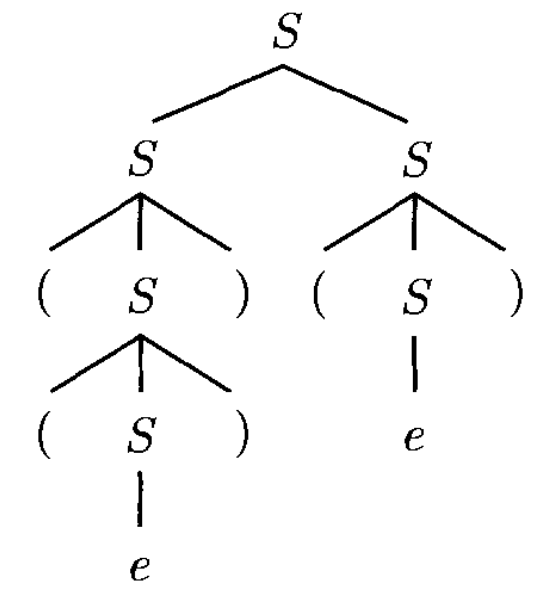
\includegraphics[width=.2\textwidth]{img/fig3-4.png}
        \caption{}
    \end{figure}
\end{example}

\begin{multicols}{2}
\setlength{\columnsep}{1.5cm}
\setlength{\columnseprule}{0.2pt}
    
We say that two derivations $D$ and $D'$ are \textbf{similar} if the pair $(D, D')$ belongs in the \textit{reflexive, symmetric, transitive closure} of $\prec$. Since the reflexive, symmetric, transitive closure of any relation is by definition reflexive, symmetric, and transitive, similarity is an equivalence relation. To put it otherwise, two derivations are similar if they can be transformed into another via a sequence of ``switchings'' in the order in which rules are applied. Such a ``switching'' can replace a derivation either by one that precedes it, or by one that it precedes.

Each equivalence class of derivations under similarity, that is to say, each parse tree, contains a derivation that is \textit{maximal} under $\prec$; that is, it is not preceded by any other derivation. This derivation is called a \textbf{leftmost derivation}. A leftmost derivation exists in every parse tree, and it can be obtained as follows. Starting from the label of the root $A$, repeatedly replace the \textit{leftmost nonterminal in the current string} according to the rule suggested by the parse tree. Similarly, a \textbf{rightmost derivation} is one that does not precede any other derivation; it is obtained from the parse tree by always expanding the \textit{rightmost nonterminal in the current string}. \textit{Each parse tree has exactly one leftmost and exactly one rightmost derivation}. This is so because the leftmost derivation of a parse tree is uniquely determined, since at each step there is one nonterminal to replace: the leftmost one. Similarly for the rightmost derivation.

It is easy to tell when a step of a derivation can be a part of a leftmost derivation: the leftmost nonterminal must be replaced. We write $x \xRightarrow[]{L} y$ if and only if $x = wA\beta$, $y = w\alpha\beta$, where $w \in \Sigma^*$; $\alpha, \beta \in V^*$; $A \in V - \Sigma$; and $A \ra \alpha$ is a rule of $G$. Thus, if $x_1 \Ra x_2 \Ra \cdots \Ra x_n$ is a leftmost derivation, then in fact $x_1 \xRightarrow[]{L} x_2 \xRightarrow[]{L} \cdots \xRightarrow[]{L} x_n$ Similarly for rightmost derivations (the notation is $x \xRightarrow[]{R} y$).

To summarize our insights into parse trees and derivations in this section, we state without formal proof the following theorem.

\begin{theorem}{}
    Let $G = (V, \Sigma, R, S)$ be a context-free grammar, and let $A \in V - \Sigma$, and $w \in \Sigma^*$. Then the following statements are equivalent:
    \begin{itemize}
        \item $A \Ra^* w$.
        \item There is a parse tree with root $A$ and yield $w$.
        \item There is a leftmost derivation $A \xRightarrow[]{L}^* w$.
        \item There is a rightmost derivation $A \xRightarrow[]{R}^* w$. 
    \end{itemize}
\end{theorem}

\subsection{Ambiguity}

There may be a string in the language generated by a context-free grammar with two derivations that are \textit{not similar} -that is to say, with two distinct parse trees, or, equivalently, with two distinct rightmost derivations (and two distinct leftmost derivations).

Given a grammar $G = (V, \Sigma, R, S)$, if a string $w \in L(G)$ has two different parse trees (two different derivations that are not similar), then the grammar is called \textbf{ambiguous}. Assigning a parse tree to a string is called ``\textit{parsing}''. It is an important concept since parsing allows us to understand why the string belongs to the grammar. In addition, it gives a ``\textit{meaning}'' (or \textit{interpretation}) to the string, which is particularly important for the programming languages.

A context-free language $L$ is called \textbf{inherently ambiguous} if every grammar $G$ that generate $L$, i.e. $L = L(G)$, is \textit{ambiguous}.

\end{multicols}
